\section{Test Results}\label{cha:TestProcedure}

\begin{table}[H] \centering
\begin{tabular}{|p{1cm}|p{12cm}|p{2cm}|}
\hline%-----------------------------------------------------------------------------------------------------------------
\textbf{Req. no.}  &  \textbf{Results} &  \textbf{Fulfilled?}         \\
\hline%-----------------------------------------------------------------------------------------------------------------
           1    &   The received coordinates from the GoT system is compared to the log file from the GoT system, shown in \tableref{AccT1tab}. All the coordinates is equal to the coordinates measured and send from the GoT and the coordinates have be received correctly.    &   Yes               \\
\hline%-----------------------------------------------------------------------------------------------------------------
           2    &   The packages, including the error packages, that the GoT system send, is received by the Arduino, where the error handling parts of the protocol filter all the error packages away, shown in \tableref{AccT2tab}.   &  Yes                \\
\hline%-----------------------------------------------------------------------------------------------------------------
           3    &   The speed between the positions, measured by the GoT system is shown on \figref {AccT3fig}, where the packages send to the Arduino is green and those that is not send is red. All positions, that have moved away faster than 3 $m \cdot s^{-1}$ is not send.   &  Yes            \\
\hline%-----------------------------------------------------------------------------------------------------------------
           4    &   Test not made   &   No                \\
\hline%-----------------------------------------------------------------------------------------------------------------
           5    &   The vehicle is running, until the power supply is adjusted down to 6V, where vehicle stops running. &   Yes              \\
\hline%-----------------------------------------------------------------------------------------------------------------
           6    &   As the steering controller do not work, as the magnetometer do not work in the room with the GoT system, the test could not be performed normally. Instead the vehicle is moved around manually, where the coordinates and the current line is monitored on a computer, which is shown on \figref{AccT6fig}. The figure shows that the route controls sets new line correctly and the requirement should be fulfilled with a working steering controller.  &    No                \\
\hline%-----------------------------------------------------------------------------------------------------------------
           7    &   As the steering controller do not work, as the magnetometer do not work in the room with the GoT system, the test could not be performed normally. Instead the vehicle is placed with a distance of 1 m away from the route line and then manually moved closer to the line, while the distance controller and error distance is monitored, which is shown on \figref{AccT7fig}. This shows that the controller behaved as planned and the requirement should be fulfilled with a working steering controller.   &   No            \\ 
\hline%-----------------------------------------------------------------------------------------------------------------
           8    &   The vehicle is set to drive 1,4 $m \cdot s^{-1}$ uphill and downhill, which is shown on \figref{AccT8Ufig} and \figref{AccT8Dfig} respectively. The figures shows the controller keeping the speed on 1,4 $m \cdot s^{-1}$.  &    Yes              \\
\hline%-----------------------------------------------------------------------------------------------------------------
\end{tabular}
\label{tab:AcceptTestTestResults}
\end{table}


%%% Test 1 %%%
\begin{table}[H]
\centering
\begin{tabular}{|l|l|l|}
\hline
GoT log file & Arduino received & Equal? \\
\hline
53,-23,-271 & 53,-23,-271 & Yes \\
\hline
53,-24,-264 & 53,-24,-264 & Yes \\
\hline
53,-24,-269 & 53,-24,-269 & Yes \\
\hline
55,-24,-267 & 55,-24,-267 & Yes \\
\hline
55,-23,-269 & 55,-23,-269 & Yes \\
\hline
56,-23,-274 & 56,-23,-274 & Yes \\
\hline
57,-22,-274 & 57,-22,-274 & Yes \\
\hline
59,-21,-274 & 59,-21,-274 & Yes \\
\hline
57,-22,-270 & 57,-22,-270 & Yes \\
\hline
55,-23,-269 & 55,-23,-269 & Yes \\
\hline
\end{tabular}
\label{AccT1tab}
\caption{The coordinates send form the GoT system to the Arduino, where all 10 sets of coordinates is equals to each other.}
\end{table}

%%% Test 2 %%%
\begin{table}[H]
\centering
\begin{tabular}{|p{3cm}|p{8cm}|p{4cm}|}
\hline
Package & Error & Returned error value \\
\hline
240,128,224,28, 128,6,80,33 ,216,98,169,15 & None & 0 \\
\hline
240,128,96,27, 0,7,144,33, 216,222,192,15 & None & 0 \\
\hline
240,128,96,28, 192,6,33,216, 30,177,15 & In the first package, there is missing a byte. The second package's first byte will be read as the 12th byte in the first package & 5,1,1,1,1,1,1,1,1,1,1,1 \\
\cline{1-1}
240,128,96,27, 0,7,144,33, 216,222,192,15 & & \\
\hline
240,128,96,28, 192,6,240,33, 216,24,177,15 & None & 0 \\
\hline
240,128,96,126, 192,6,16,34, 216,22,193,15 & Byte 4 is changed & 4 \\
\hline
240,128,96,28, 192,6,80,34, 216,18,177,15 & None & 0 \\
\hline
26,128,96,28, 192,6,48,34, 216,20,177,15 & Byte 1 is changed & 1,1,1,1,1,1,1,1,1,1,1,1 \\
\hline
240,128,96,28, 192,6,240,33, 216,24,177,15 & None & 0 \\
\hline
240,128,96,28, 128,6,208,63, 33,216,90,177, 15 & The package contains a byte to much. The system will see the first 12 bytes as a package and 12th byte as the start of a new package. & 5,1 \\
\hline
240,128,96,28, 192,6,144,33, 216,30,177,15 & None & 0 \\
\hline
240,128,96,28, 192,6,176,33, 216,28,177,15 & None & 0 \\
\hline
240,128,115,28, 128,6,208,33, 216,90,177,15 & Byte 3 is changed & 3,1,1,1,1,1,1,1,1,1 \\
\hline
240,128,96,29, 64,6,112,34, 216,144,161,15 & None & 0 \\
\hline
240,96,96,28, 64,6,48,34, 216,148,177,15 & Byte 2 is changed & 2,1,1,1,1,1,1,1,1,1,1 \\
\hline
\end{tabular}
\label{AccT2tab}
\caption{The packages send from the GoT system, where some packages have been force with a error. The returned error value, is the output from the error handling from the protocol. 1 is equal wrong start byte, 2 is wrong destination, 3 is wrong length, 4 is failed checksum control and 5 is wrong end byte.}
\end{table}

%%% Test 3 %%%
\begin{figure}[H]
  \centering
	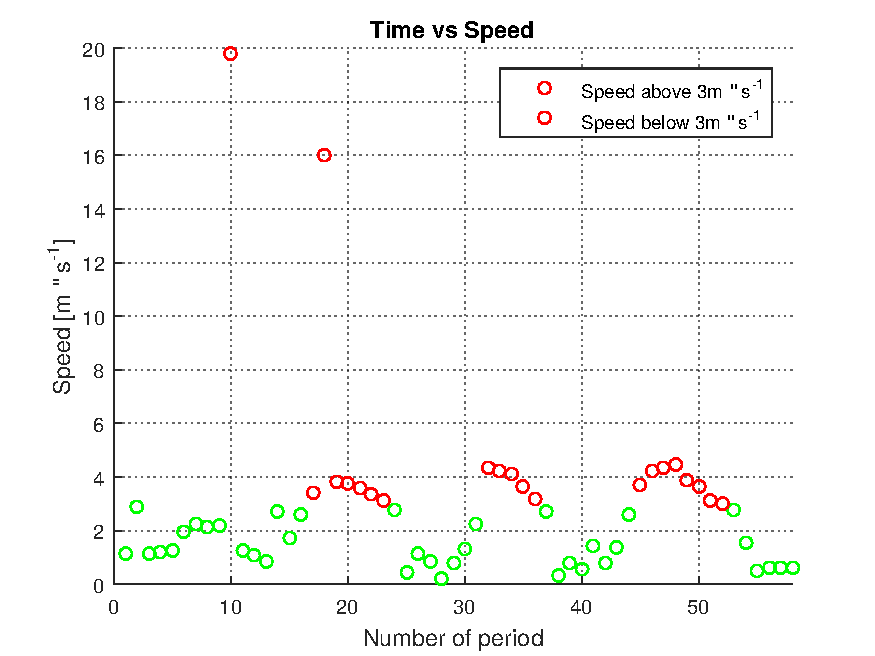
\includegraphics[scale=0.8]{figures/AccTest3.pdf}
	\caption{Plot of all the velocity between the measured positions, where the red marks indicates discarded measurements and green indicates the measurements send to the Arduino.}
	\label{AccT3fig}
\end{figure}


%%% Test 6 %%%
\begin{figure}[H]
  \centering
	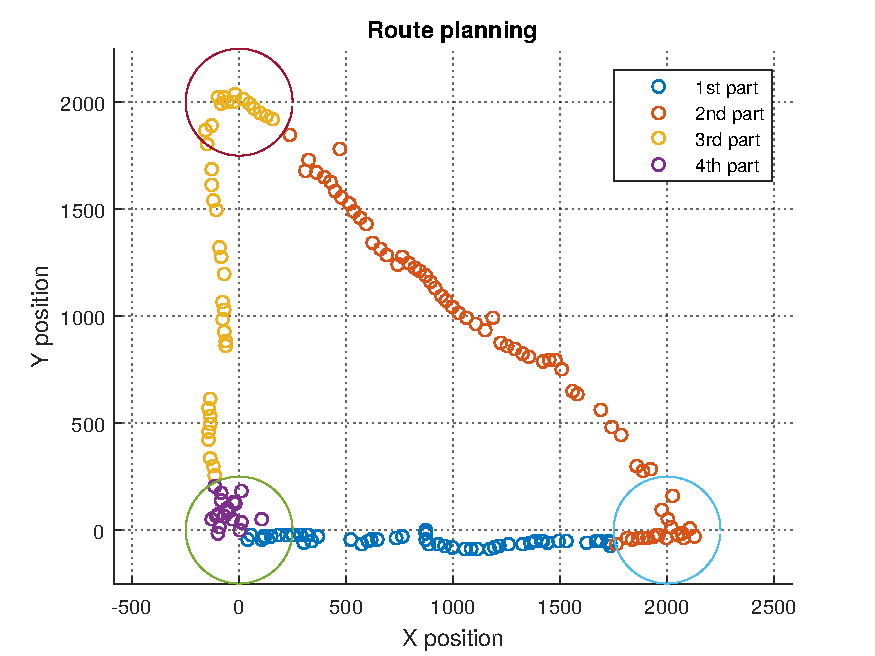
\includegraphics[scale=0.8]{figures/AccTest6.pdf}
	\caption{Plot of coordinates measured, where the different part of the route is indicated as different colours. It is seen that the route control shift to a new line, each time the vehicle is under 28 cm away from the end point.}
	\label{AccT6fig}
\end{figure}


%%% Test 7 %%%
\begin{figure}[H]
  \centering
	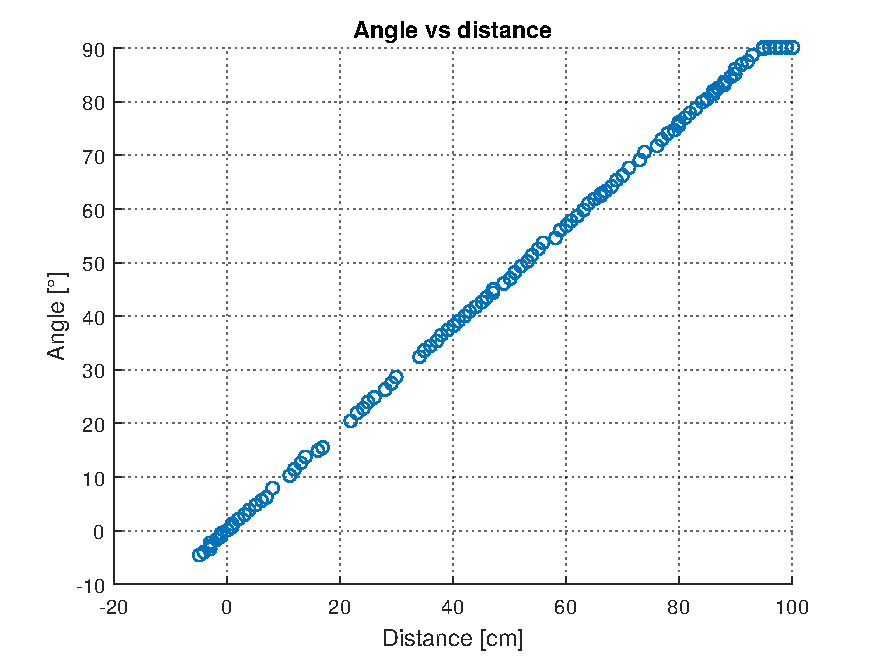
\includegraphics[scale=0.8]{figures/AccTest7.pdf}
	\caption{Plot of the angle output from the distance controller compared to the error distance. It is seen that the angle gets smaller, thus smaller the error distance is.}
	\label{AccT7fig}
\end{figure}

%%% Test 8 %%%
\begin{figure}[H]
  \centering
	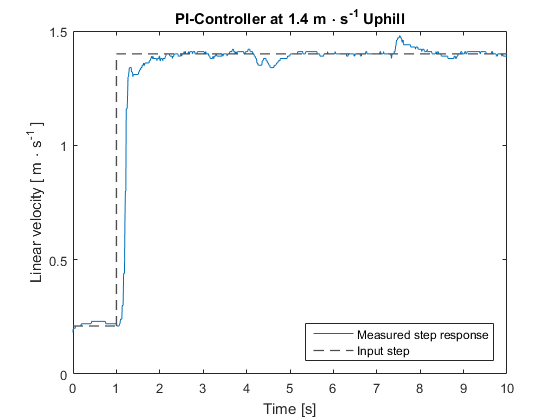
\includegraphics[scale=0.8]{figures/AccTest8U.png}
	\caption{Step response for the vehicle, where the vehicle hits a uphill ramp after 4 seconds and hits flat terrain again after 7,5 second.}
	\label{AccT8Ufig}
\end{figure}

\begin{figure}[H]
  \centering
	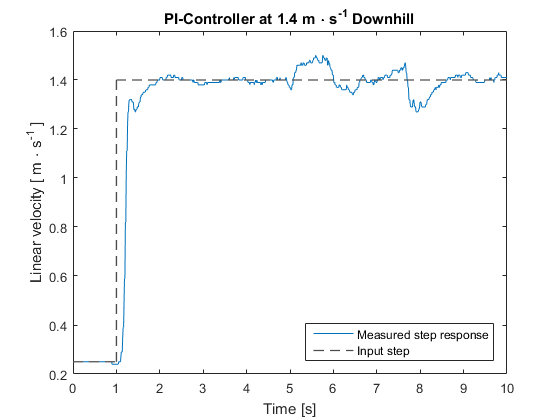
\includegraphics[scale=0.8]{figures/AccTest8D.png}
	\caption{Plot of all the velocity between the measured positions, where the red marks indicates discarded measurements and green indicates the measurements send to the Arduino.}
	\label{AccT8Dfig}
\end{figure}